\documentclass{report}
\usepackage{graphicx}
\usepackage{lipsum}  
\usepackage{hyperref}
\usepackage{listings}
\usepackage{xcolor}
\usepackage{here}

\usepackage{biblatex}
\addbibresource{proposalReferences.bib}


\title{Project Proposal}
\author{Rodrigo Almeida}
\date{\today}

\begin{document}

\maketitle
\chapter{Project Proposal}
\textbf{Supervisor:} Dr. Damien Costello\par
\noindent\textbf{Project Name:} Biometric Data Analysis in Digital Game Scenario

\section*{Project Context}
\subsection*{Introduction}
\par

\textbf{PUBG:} PUBG, short for PlayerUnknown's Battlegrounds, is a popular online multiplayer battle royale game developed and published by PUBG Corporation, a subsidiary of Bluehole Studio. In PUBG, up to 100 players parachute onto an island and scavenge for weapons and equipment to kill others while avoiding getting killed themselves. The game features a shrinking safe area to force players into close encounters, promoting tactical gameplay and intense firefights. The last player or team standing wins the game. PUBG became widely popular upon its release in 2017 and is available on various platforms, including PCs, consoles, and mobile devices1.\cite{PUBG}.
\par 
Since its launch in 2017, PUBG has become incredibly popular, with more than 280M active players \cite{PUBG_users}. People of all ages and from all over the world enjoy playing this game. In PUBG, players need good hand-eye coordination and quick reflexes to compete well against others. The game offers a variety of weapons, and players can customize their controls to fit their preferences. This project builds upon the research done by university students, focusing on collecting biometric data to improve player performance in digital games~\cite{PUBG}.

\subsection*{Previous Project}
The original project, titled \textbf{"Biometric Data Collection for Performance Optimization in a Digital Game Scenario"}, aimed to find out if a player's body data could help them play a video game better. The researchers set up a practice game similar to PUBG: Battlegrounds, with the same weapons and controls in a Unity Desktop {\tt Application}. Biometric data was supplied by a {\tt Smart Watch}. The goal was to see if there was a connection between how players performed in the game and their body data.

\par
In our third-year project, our team was given the challenge of enhancing the visualization of data from both the test games and the Polar API. To achieve this, we developed a chart API, enabling users to conveniently view all the results on a single page. The chart API was specifically created to present the data collected during the initial research in a coherent and user-friendly chart format, integrating various user data into one unified visual representation.

\section*{Project Objective}
The aim of this research project is to overcome the limitations mentioned in previous projects and complete the future development goals of both projects.
These include:

\begin{itemize}
\item {Chart API Integration}\\
Integration of developed Chart API into the test application.
\item {Offline Data Storage}\\
Provision will be made for offline temporary file storage to improve the overall reliability of the whole system
\item{PUBG API}\\
Further research on new developments in the PUBG API for better user experience. 
\end{itemize} 
        
And eventually, seek to answer the following research questions:
\begin{itemize}
\item {Can the user's current physical condition as indicated by their Biometric data, have any direct relationship with their performance in such a gaming scenario?}
\item {Can Biometric and test data help suggest the most suitable settings for different game scenarios?}
\end{itemize}

\section*{Technologies \& System Architecture}
\subsection*{Legacy Architecture}

The entire system architecture, as designed in the previous projects, is visualized in \autoref{fig:systemArchitecture}. This system consists of three modules that interact with both an external API and user devices. These modules are detailed as follows:

\begin{itemize}
\item{Test Application}\\
A Unity-designed desktop application on a Windows Platform where users can play tests for different game scenarios.
\item {Node Js Web Application}\\
An Express Node JS Web application deployed on Amazon EC2 Virtual machine, serving as a callback endpoint for OAuth 2.0 Authentication for the Polar Flow API. 
\item {Firestore Data Storage}\\
Permanent storage medium for user's test and Biometric data.
\end{itemize}
User Devices:
\begin{itemize}
\item{Smart Watch}
\item {Smart Phone}
\end{itemize}

\begin{figure}[h]
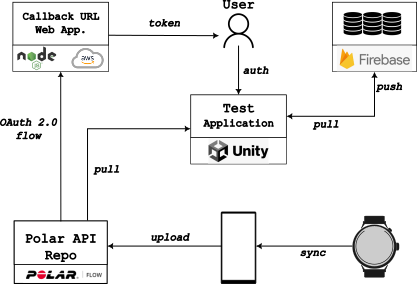
\includegraphics{images/architecture.png}
\caption{System Architecture}
\label{fig:systemArchitecture}
\centering
\end{figure}

The actions in the Figure \autoref{fig:systemArchitecture} can be summarized as follows:
\begin{itemize}
\item{sync}: passing of biometric data to a smartphone from a Polar watch.
\item {upload}: uploading of biometric data to Polar API repository.
\item {OAuth 2.0 flow}: Multi step OAuth 2.0 authentication protocol. 
\item {token}: getting verification token from the Callback URL by the user.
\item {pull (Polar API - Test Application)}: retrieving biometric data from Polar API by the Test Application.
\item {auth}: The user supplies a token to the Test Application as a final step of authentication. 
\item {pull (Firebase - Test Application)}: retrieving user test/biometric data for rendering by Test Application.
\item {push}: saving user's test/biometric data to a Datastore.
\end{itemize}


\subsection*{Proposed Architecture}
The final system architecture will include new modules to facilitate data analytics using AI models. The new system calls for a relational database replica of the Firebase storage to ensure data consistency, predictability and structures suitable for relevant statistical analysis. A.I models as a mini-service that performs operations with supplied data and returns the result of the analysis. A Web Application that functions as a Controller that interfaces the data and A.I modules, Executive Dashboard that renders user data and results from the A.I models and any other information about the system.\\
\autoref{fig:proposed_web_architecture} shows the proposed architectural layout for the System.\\


\begin{figure}[h]
    \centering
    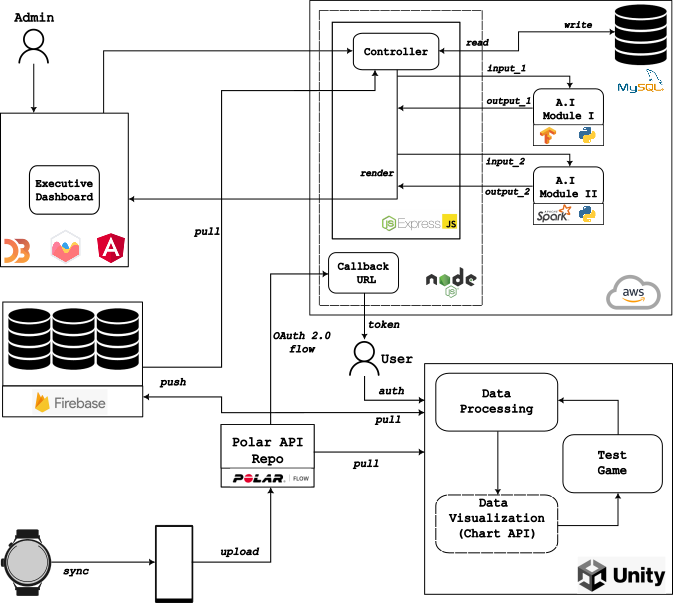
\includegraphics[scale=0.68]{images/new-arch.png}
    \caption{Web Application Architecture}
    \label{fig:proposed_web_architecture}
\end{figure}


Additional modules have been added to the web application namely back end `Controller' \& front end `Executive Dashboard', and a 'Relational Database'. The functions of these modules are explained below:

\begin{itemize}
\item {Controller}: This module is responsible for coordinating data fetch from the Relational Database and making sure that the Relational Database is always in sync with the Firebase Datastore. It is also responsible for filtering and structuring data being fed into the A.I. Modules and when necessary using the output for an A.I module as input for another A.I module. 
\item{Executive Dashboard}: This module provides a Graphical User Interface that displays the working dataset, and offers interfaces to filter, tune and if needed bias the data being sent to the A.I Modules for analysis. This module will developed using the Angular Framework with integration of D3.js or Chart.js for displaying relevant charts. The choice for Angular Framework over other solutions namely ReactJS and Vue is because of the more structured Angular Framework which is more suited for collaborative work.
\item{A.I Modules}: These modules are responsible for running analysis on data. The modules accept input from the `Controller' and output a comprehensive summary of the results of the analysis done to the `Executive Dashboard' module. For this purpose, TensorFlow and Apache Spark were chosen for the following reasons:
\end{itemize}

\begin{itemize}
    \item {Capabilities}: Apache Spark is capable of performing linear and logical regression\cite{apache_spark} which are common tools used for this class of problem. TensorFlow also has the same capabilities and can perform regression neural network models\cite{tensor_flow}.
    \item {Accessibility}: Both tools are open-source and available to the general public\cite{open_source}.
    \item{Python API interface}: Both tools provide a Python API. This eases deployment as Python is platform-independent and relatively easy setup in a Ubuntu Virtual machine.
    \item{Large Community}: Both have a large community of contributors. Documentation and tutorials are vastly available on the internet.
    \item{Relational Database}: Data for the analysis will be sourced directly from this Database which is a structured replica of the FireStore Database as obtained from the Legacy System. The rationale for this Module is to provide a flexible means of retrieving data in various forms and shapes as may be needed for analysis and also overcome the high complexities involved in FireStore for compound queries.
    \item{Chart API}:
    Is responsible for displaying test results and biometric data to the users. This already developed module will be integrated into the 'Test Application' and undergo some modification to be able to display custom data as requirements change. 
    
\end{itemize}

\subsection*{Schedule of Work}
As this project is mainly a Research Project, my project partner and I will be actively engaging in gathering, and analysing relevant data. By conducting research we aim to contribute to the project's overall success.

Regarding the tasks that will be carried out, it will be divided as follows:

\begin{itemize}
    \item {Controller}: Otito
    \item {Executive Dashboard}: Rodrigo
    \item {AI Module I}: Rodrigo
    \item {AI Module II}: Otito
    \item {Database Design}: Rodrigo and Otito 
\end{itemize}

To ensure we effectively manage our project we have explored a few options and decided to use  Jira software for planning and tracking our project sprints. However, we can adapt to other tools as the project evolves. As part of our research, we are also exploring GitHub for project management. Depending on our project requirements, we are open to transitioning to GitHub as our project management tool if it proves to be a more suitable and efficient option. Our flexibility reflects our commitment to find not only the most effective tools but also tools that we didn't use before aiming the project's success.

The project will be broken down into multiple sprints. At the end of each sprint, we will conduct a retrospective meeting to evaluate progress and identify areas for improvement.\\
\autoref{fig:Project_Schedule} shows the overall planned schedule for the project from group formation up to the Project submission. \\
Additionally, the project schedule are further elaborated below:\\
\autoref{fig:Project_Init} shows the schedule for the Environment to be set up.\\
\autoref{fig:Env_Setup} shows schedule for Project Initialization. \\
\autoref{fig:dash_design}  shows the schedule for the Executive Dashboard to be finalized. \\
\autoref{fig:ai_deploy} shows the schedule for the AI module to be deployed. \\
\autoref{fig:review_deploy} shows the schedule for Design Review, Completion of AI model and Dashboard, Refactoring Integration, and Deployment.\\
\autoref{fig:final} finally shows the schedule for the Final Dissertation and Project submission.\\

\begin{figure}[h]
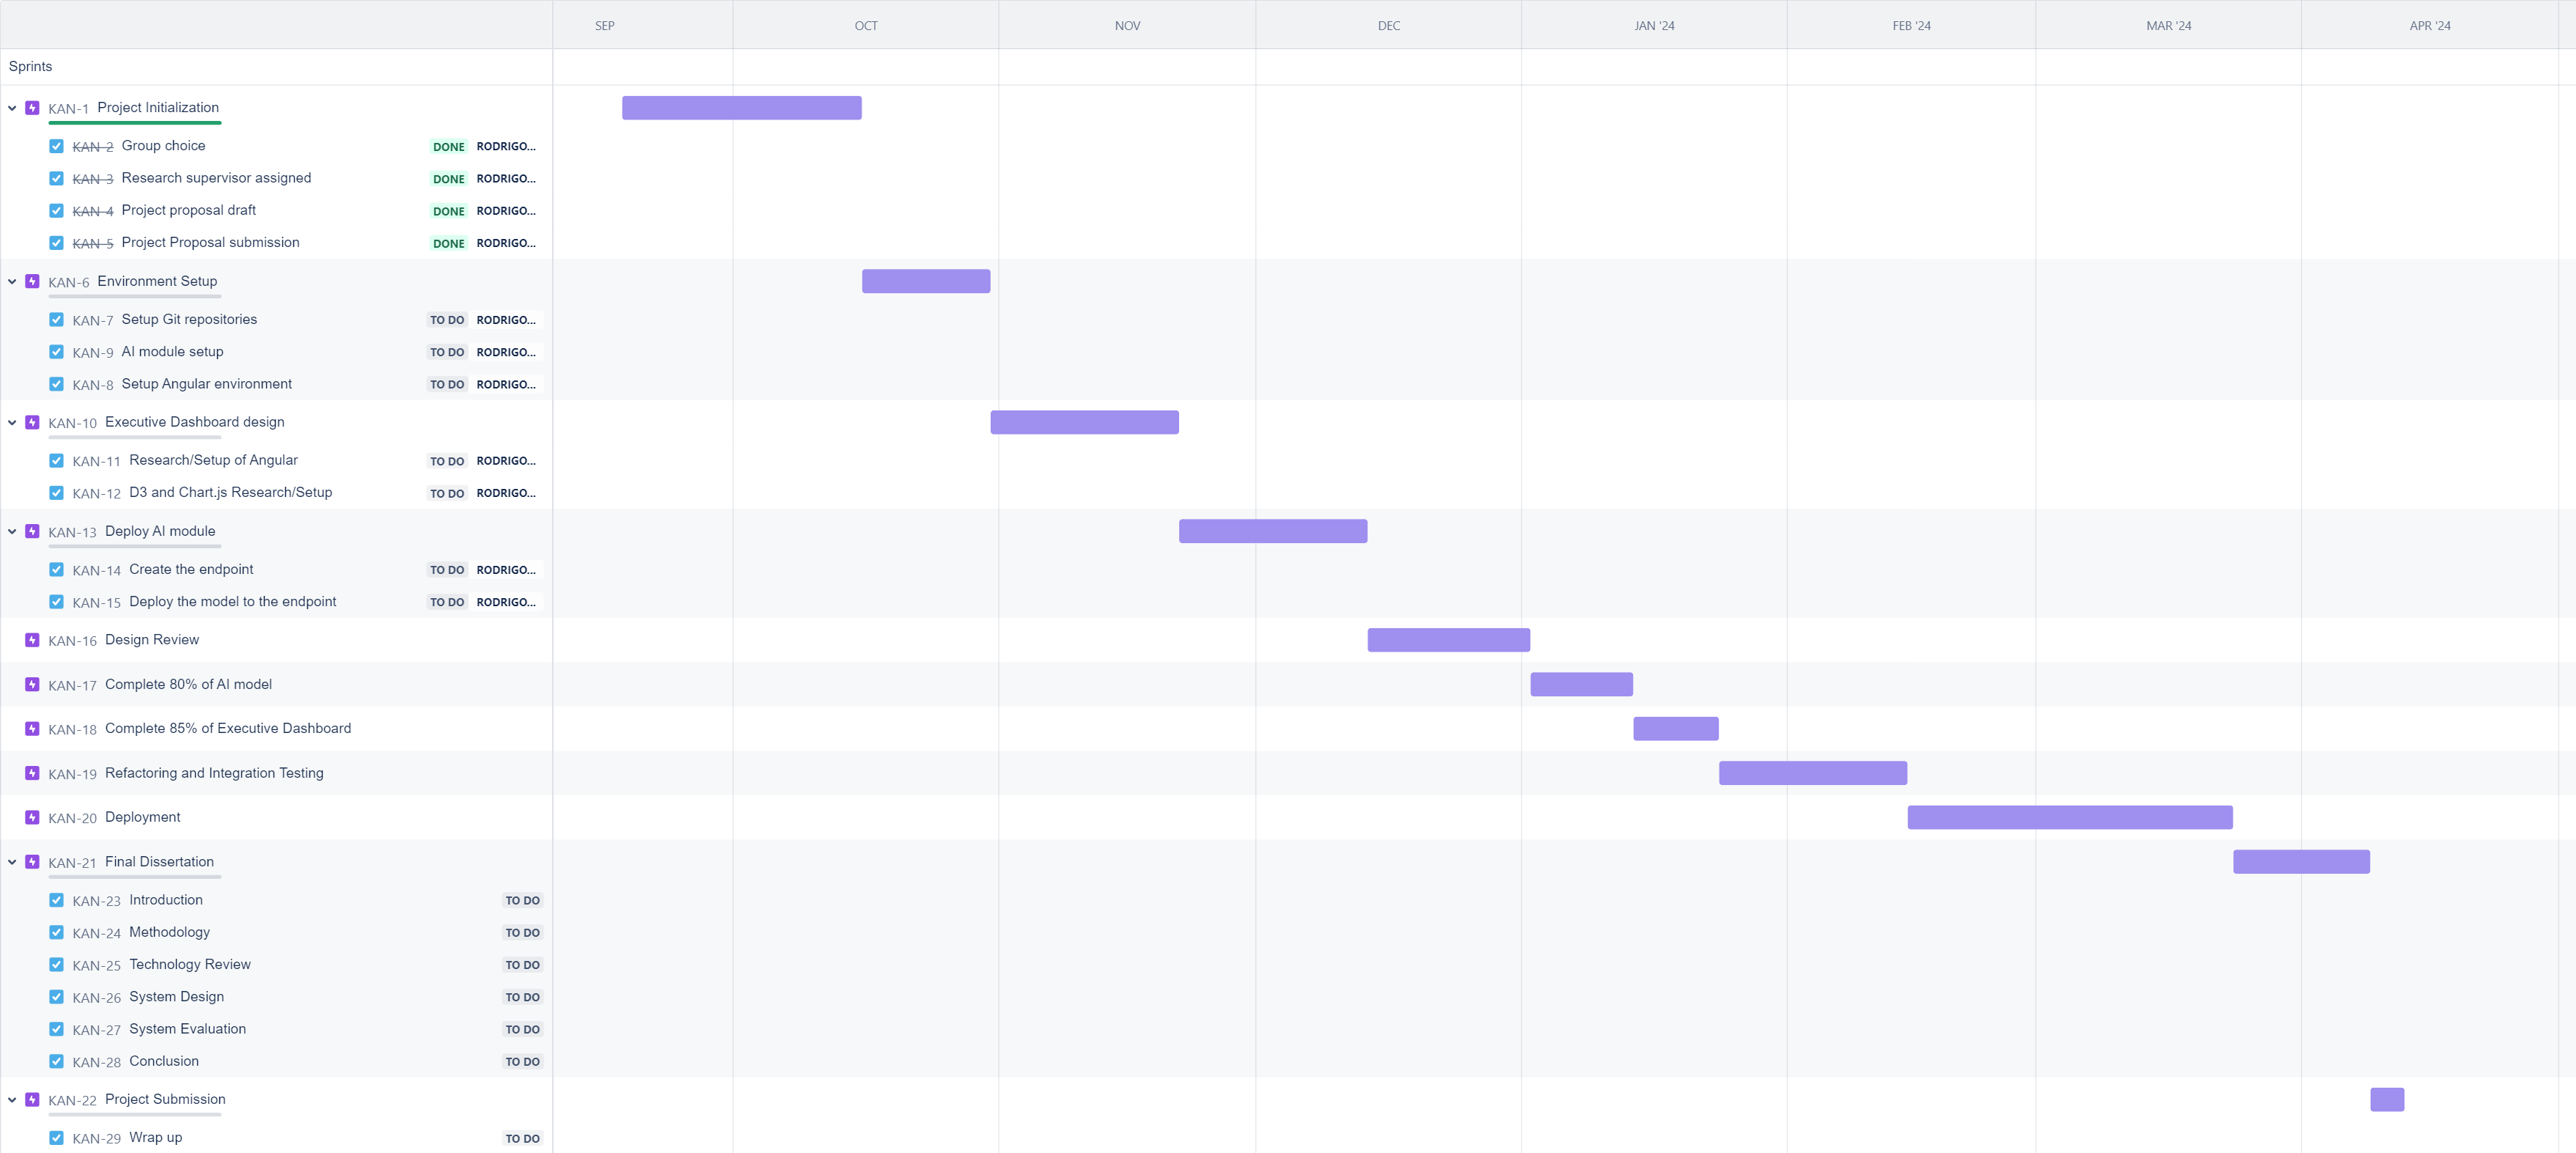
\includegraphics[scale=0.1]{images/gantt.png}
\caption{Gantt Chart - Overall Project Schedule}
\label{fig:Project_Schedule}
\centering
\end{figure}


\begin{figure}[h]
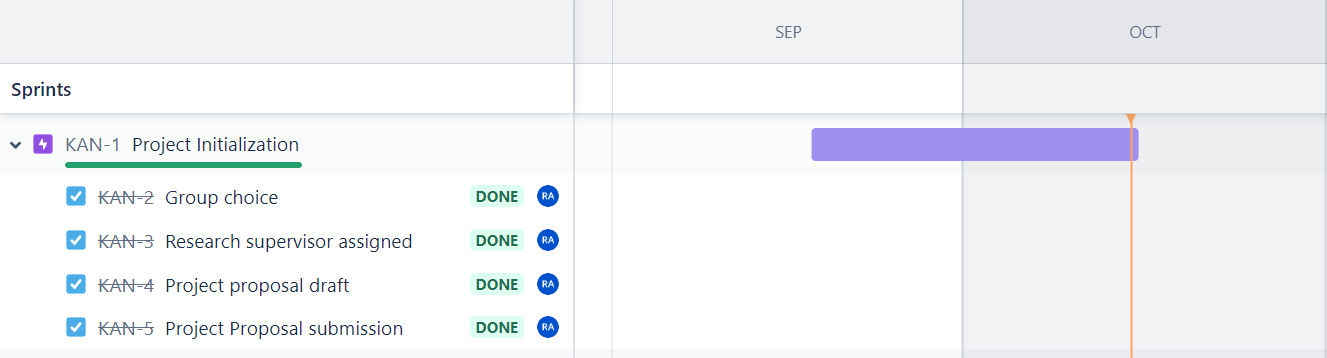
\includegraphics[scale=0.49]{images/gantt/project_init.png}
\caption{Gantt Chart - Project Initialization}
\label{fig:Project_Init}
\centering
\end{figure}

\begin{figure}[h]
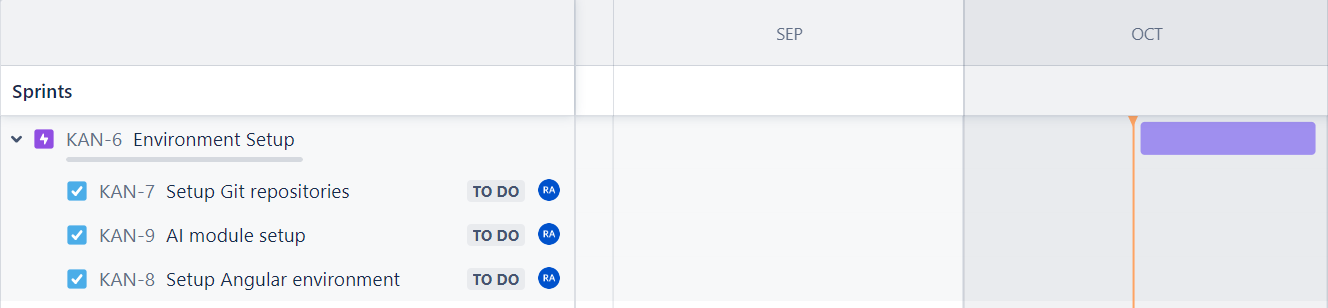
\includegraphics[scale=0.49]{images/gantt/env_setup.png}
\caption{Gantt Chart - Environment Setup}
\label{fig:Env_Setup}
\centering
\end{figure}


\begin{figure}[h]
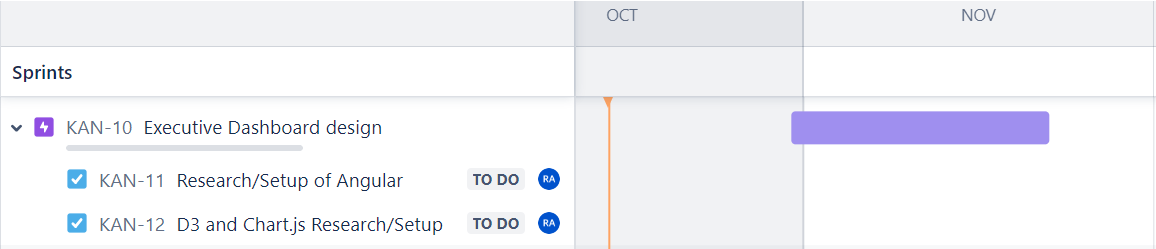
\includegraphics[scale=0.49]{images/gantt/dash_design.png}
\caption{Gantt Chart - Dashboard Design}
\label{fig:dash_design}
\centering
\end{figure}


\begin{figure}[h]
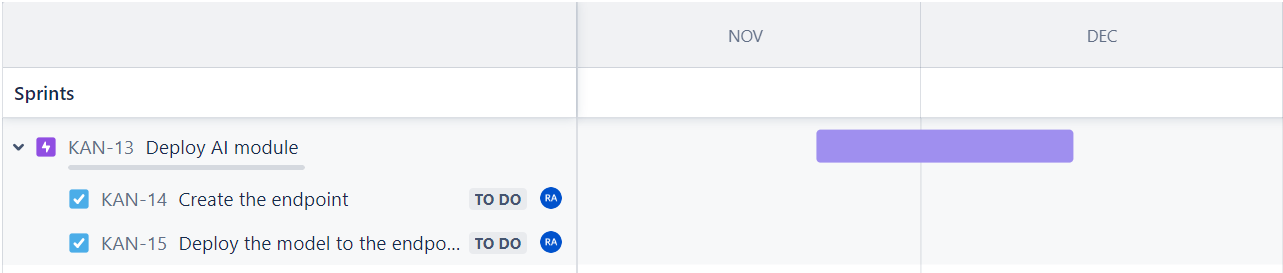
\includegraphics[scale=0.49]{images/gantt/ai_deploy.png}
\caption{Gantt Chart - AI Module Deployment}
\label{fig:ai_deploy}
\centering
\end{figure}


\begin{figure}[h]
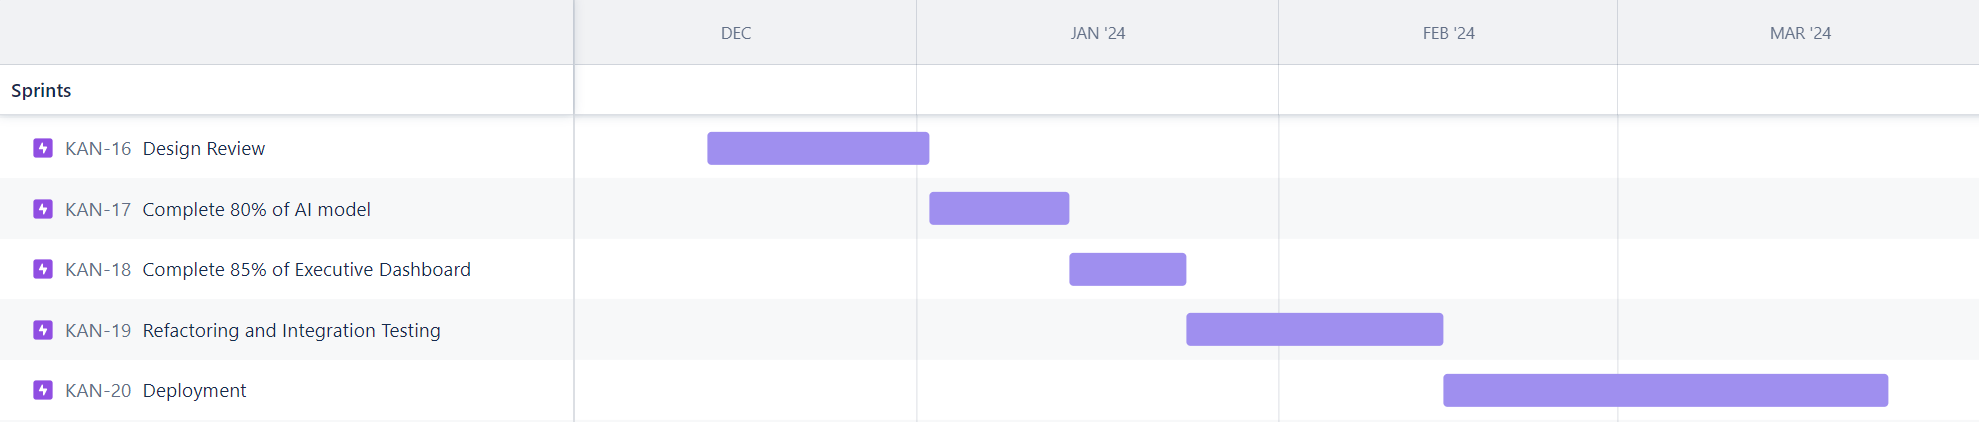
\includegraphics[scale=0.32]{images/gantt/review_deploy.png}
\caption{Gantt Chart - Design Review, Completion of AI model and Dashboard, Refactoring and Integration, Deployment}
\label{fig:review_deploy}
\centering
\end{figure}

\begin{figure}[h]
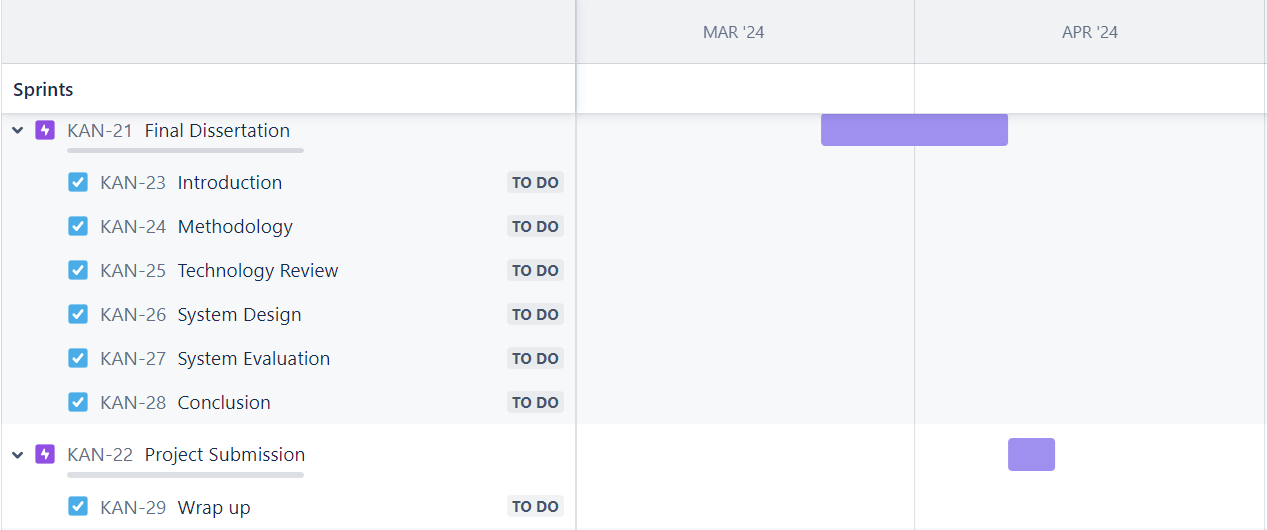
\includegraphics[scale=0.50]{images/gantt/final.png}
\caption{Gantt Chart - Final Dissertation and Project Submission}
\label{fig:final}
\centering
\end{figure}


\printbibliography



\end{document}

